\section{Results}

\subsection{Integrity checks and aggregate accuracy}

The confirmatory analyzer accepted the complete grid of \ConfirmatoryRuns{}
trained models and \ConfirmatoryTrajectories{} trajectory-level rows. All
prespecified metrics were finite (\AllMetricsFinite), and the 40 seed--system
groups produced \UniqueDataHashes{} distinct data fingerprints while sharing
one fingerprint across methods within each group. These checks establish grid
completeness and pairing; they are not performance evidence.

Table~\ref{tab:main-results} reports the seed-balanced mean and standard
deviation for horizons 1, 10, and 25. Across all 11 methods, \BestMethod{}
had the lowest aggregate NRMSE-25 (\BestNRMSE). CFR-WM's mean was
\CFRNRMSE{}, compared with \PGNNNRMSE{} for the preselected PGNN-style comparator.
This ordering is descriptive: confirmatory support depends on paired
seed-level effects and frozen practical margins, not on the lowest pooled mean
alone.
The confirmatory estimand does not follow solely from these pooled means: it
averages eight within-seed relative effects after giving every fixed
system--regime cell equal weight.

\begin{table*}[t]
\centering
\caption{Confirmatory accuracy over the fixed five-system, three-regime
benchmark. Entries are means $\pm$ SD across eight seed-level, cell-balanced
aggregates. Bold marks the lowest aggregate NRMSE-25; it does not by itself
denote confirmatory support. Parameter counts are means over the five
system-specific input dimensions; all methods received the same six-trial
validation search budget.}
\label{tab:main-results}
\resizebox{\textwidth}{!}{\input{../../results/confirmatory_analysis/table_confirmatory}}
\end{table*}

\begin{quote}
\small\textbf{Frozen primary estimand.} For each seed, PGNN-style and CFR-WM
NRMSE-25 are first averaged with equal weight over the 15 prespecified
system--regime cells; their relative improvement is then computed. The
confirmatory point estimate is the arithmetic mean of those eight seed-level
relative improvements, not the ratio of the two pooled means in
Table~\ref{tab:main-results}.
\end{quote}

\subsection{Primary and gated robustness hypotheses}

Against PGNN-style, the seed-mean relative NRMSE-25 improvement was
\PrimaryImprovement\% (95\% paired fixed-cell bootstrap CI
[\PrimaryRelativeCILow\%, \PrimaryRelativeCIHigh\%]). In absolute units,
CFR-WM minus PGNN-style was \PrimaryDifference{} (95\% CI [\PrimaryCILow,
\PrimaryCIHigh]). The exact one-sided sign-flip test against the same 5\%
practical margin gave $p=\PrimaryPValue$. Under the frozen conjunction of a
5\% interval lower bound, $p<0.05$, and finite metrics, H1 was
\PrimaryDecision. This decision is not changed by rankings against other
comparators or by favorable individual cells.

For the H2 components, the combined corrupt-ID and corrupt-OOD regimes had a
relative effect of \CorruptImprovement\% (95\% CI
[\CorruptRelativeCILow\%, \CorruptRelativeCIHigh\%], one-sided 5\%-margin
$p=\CorruptPValue$). ID-clean had an effect of \CleanImprovement\% (95\% CI
[\CleanRelativeCILow\%, \CleanRelativeCIHigh\%], one-sided signed
$-5\%$-margin $p=\CleanPValue$). Because H2 is hierarchically gated by H1 and
requires both component rules, the robustness hypothesis was
\RobustnessDecision.

Table~\ref{tab:seed-effects} exposes the eight independent cluster effects
rather than only their mean. Every seed exceeded the 5\% practical threshold,
although the exact test still treats the seed effects as the inferential units.

\begin{table}[t]
\centering
\caption{Seed-level primary effects after equal weighting of the 15 frozen
benchmark cells. Positive values favor CFR-WM.}
\label{tab:seed-effects}
\input{../table_seed_effects}
\end{table}

\begin{figure*}[t]
\centering
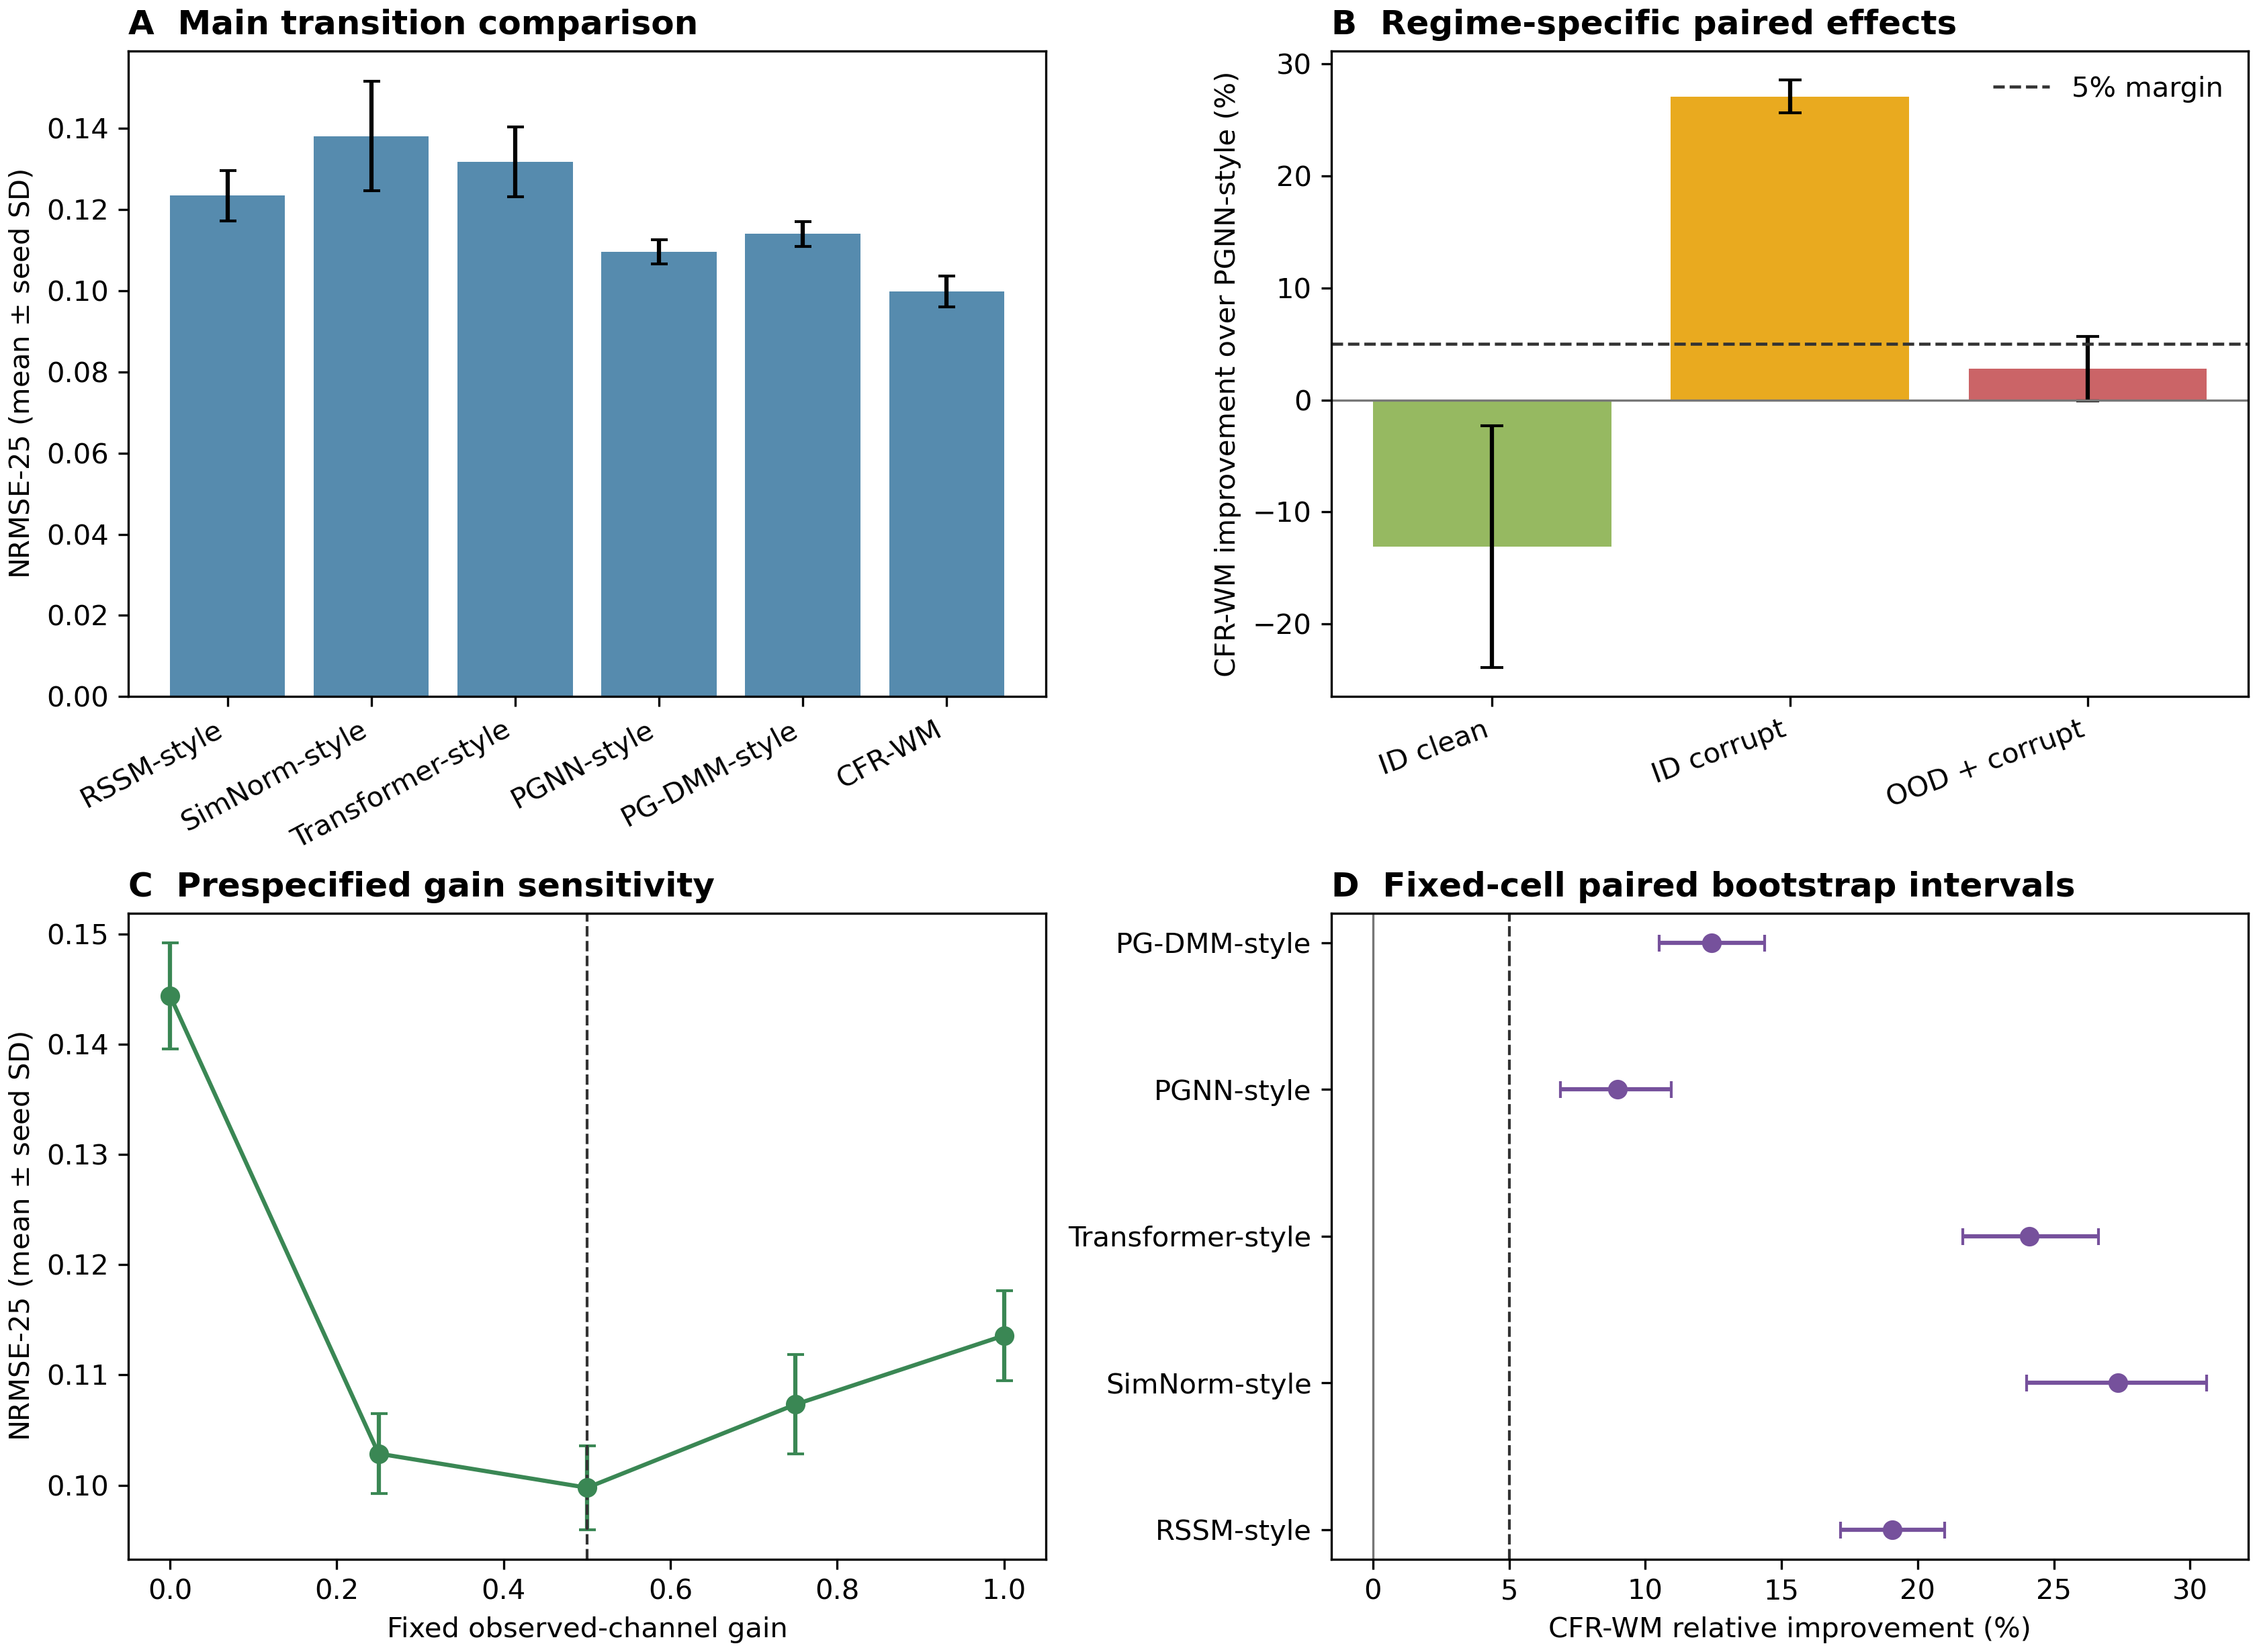
\includegraphics[width=0.96\textwidth]{figures/confirmatory_overview.png}
\caption{Locked confirmatory summary. (A) Aggregate transition accuracy for the
six main methods. (B) Paired CFR-WM effects against PGNN-style by regime; positive
values favor CFR-WM. (C) Prespecified fixed-gain sensitivity. (D) Paired
fixed-cell intervals against each broad comparator. Error bars in A--C are
seed-level SD; D uses the nested 95\% bootstrap interval.}
\label{fig:confirmatory-overview}
\end{figure*}

\subsection{Comparator and sensitivity evidence}

Table~\ref{tab:comparator-contrasts} reports every prespecified broad
comparison. Positive relative effects favor CFR-WM. The confidence intervals
retain all fixed cells, whereas the exact two-sided seed sign-flip values are
Holm-adjusted as one five-test family. These comparisons contextualize H1 but
do not replace its preselected PGNN-style contrast or its 5\% margin.

The PGNN-style row repeats the primary point estimate but uses the frozen
comparator-family bootstrap seed (20260808), whereas H1 uses its prespecified
primary seed (20260805). The estimand and 5,000-replicate resampling scheme are
otherwise identical; the separately sampled interval endpoints differ by at
most 0.01 percentage point after rounding, and only the primary interval enters
the H1 decision.

\begin{table*}[t]
\centering
\caption{CFR-WM relative NRMSE-25 effects against broad comparators. Exact
$p$ values test a zero seed-level difference; Holm adjustment is confined to
this prespecified family of five.}
\label{tab:comparator-contrasts}
\input{../table_comparator_contrasts}
\end{table*}

The lowest aggregate NRMSE-25 among gains $0$, $0.25$, $0.5$, $0.75$, and $1$
occurred at gain \BestGain. Relative to the one-step-trained variant, CFR-WM's
effect was \OneStepImprovement\% (95\% CI [\OneStepRelativeCILow\%,
\OneStepRelativeCIHigh\%], Holm $p=\OneStepHolmP$). Table
\ref{tab:sensitivity-contrasts} gives the complete second five-test family;
therefore the gain sweep is reported even when it does not favor the proposed
value.

\begin{table*}[t]
\centering
\caption{CFR-WM relative NRMSE-25 effects against gain and training-horizon
sensitivities. Positive values favor the proposed gain-0.5 multi-step model.}
\label{tab:sensitivity-contrasts}
\input{../table_sensitivity_contrasts}
\end{table*}

Secondary probabilistic metrics are shown in Table~\ref{tab:secondary}. They
are diagnostics rather than alternate confirmation endpoints: lower Gaussian
NLL, calibration error, or catastrophic-rollout rate cannot rescue a failed
H1, and diagonal-Gaussian calibration does not imply a correct joint forecast
distribution.

\begin{table*}[t]
\centering
\caption{Secondary aggregate diagnostics for the six broad methods. Rates and
scores are seed-balanced over all fixed cells and are not separately tested.}
\label{tab:secondary}
\resizebox{\textwidth}{!}{\input{../table_secondary_metrics}}
\end{table*}

\subsection{Fixed-cell heterogeneity}

Figure~\ref{fig:cell-heterogeneity} retains all 15 system--regime effects. By
the frozen descriptive guard, CFR-WM was more than 10\% worse than PGNN-style in
\CellsWorseTen{} cells. All three were ID-clean: cart--pole
(\CartpoleCleanChange\% relative change), controlled Van der Pol
(\VanDerPolCleanChange\%), and Duffing (\DuffingCleanChange\%). Conversely,
\IDCorruptFavoredCount{} of \IDCorruptCellCount{} ID-corrupt cells favored
CFR-WM, with descriptive changes from \IDCorruptLeastChange\% to
\IDCorruptMostChange\%. This pattern explains why an aggregate H1 success coexists with
failure of clean-regime noninferiority. No cell-level $p$ value is reported:
with eight seed clusters, those contrasts were not assigned confirmatory
multiplicity claims.
The exact estimates and unadjusted bootstrap intervals are archived in the
appendix table and machine-readable CSV.

\begin{figure}[t]
\centering
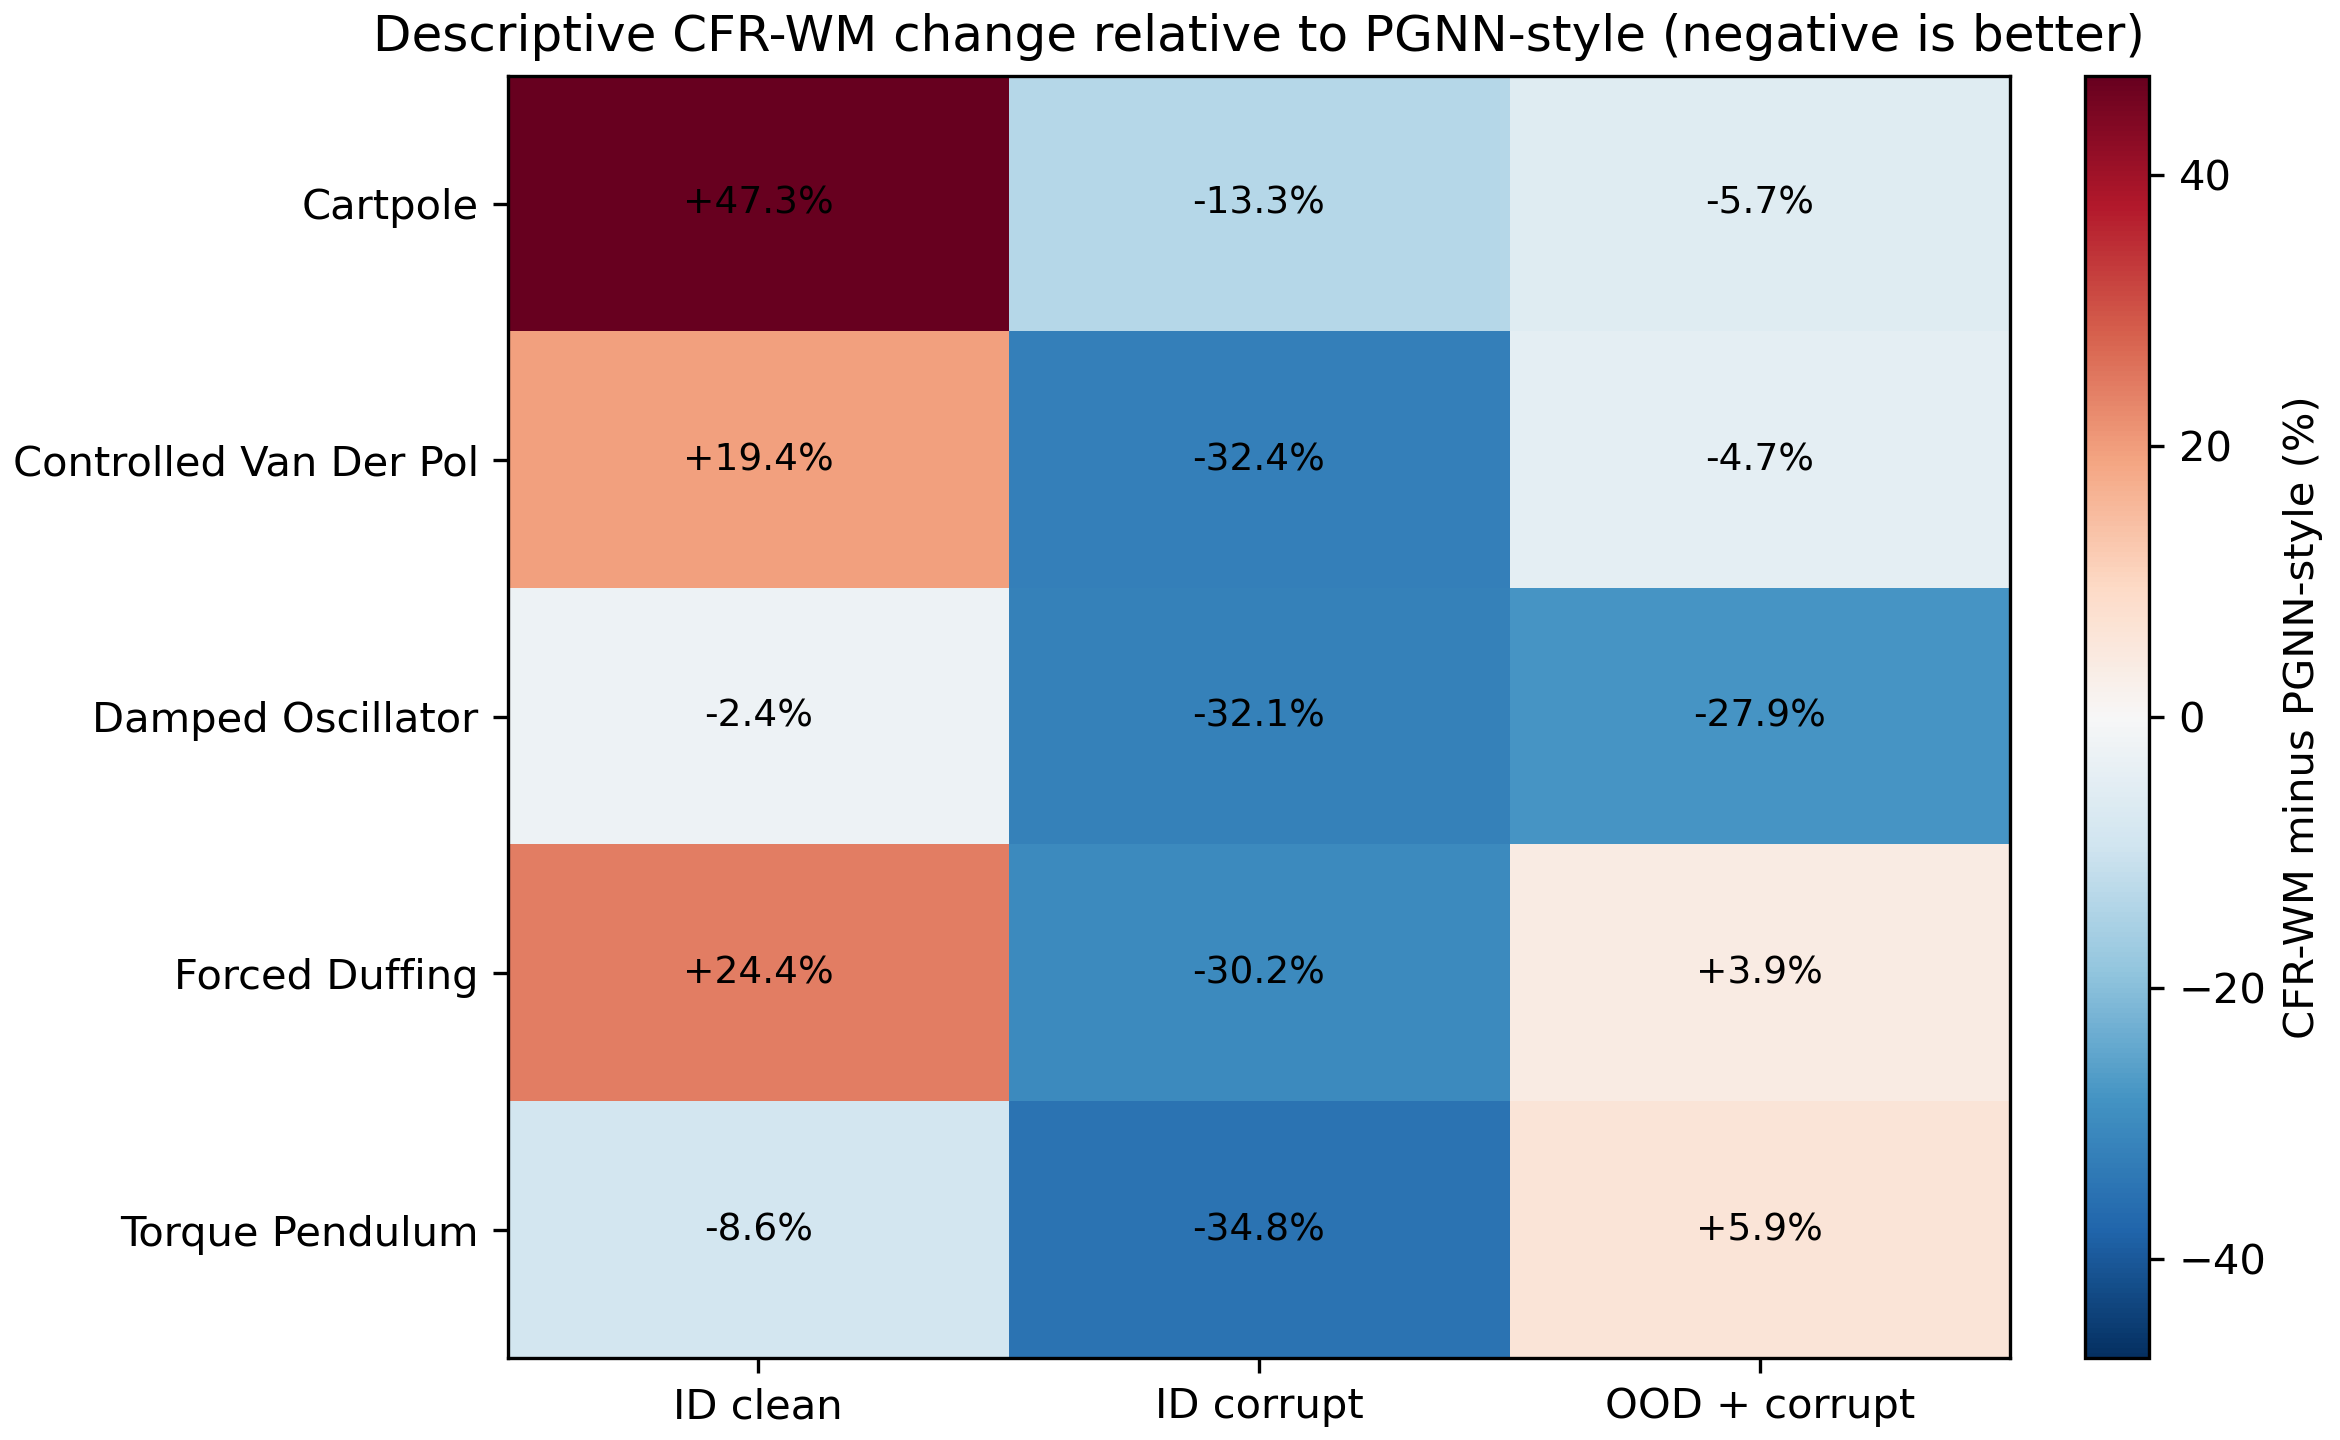
\includegraphics[width=\linewidth]{figures/cell_difference_heatmap.png}
\caption{Descriptive CFR-WM change relative to PGNN-style in each fixed benchmark
cell. Negative values mean lower NRMSE-25 for CFR-WM.}
\label{fig:cell-heterogeneity}
\end{figure}
